\section{什么是视觉风格?}
Cytoscape在网络视觉方面的一个强项就是允许用户将其数据中的各种属性(名称、类型、度、权重、基因表达数据等等)映射到视觉属性(颜色、大小、透明度、字体等等)上。这种映射关系的集合就被称为\textbf{视觉风格(Visual Style)},可以用\textbf{VizMapper}创建或编辑视觉风格。
在VizMapper中可以很方便的修改网络的外观。例如:
\begin{itemize}
\item 设定所有节点的缺省颜色和形状。 \begin{itemize}
\item \centerline{
 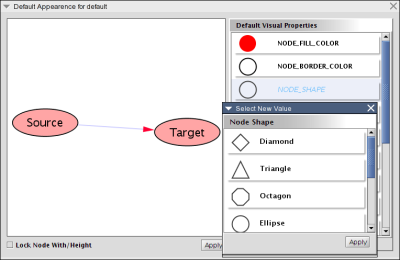
\includegraphics[width=.6\textwidth]{images/DefaultColorAndShape.png} }
\end{itemize}

\item 用不同类型的线条表示不同类型的相互作用。\begin{itemize}
\item \centerline{
 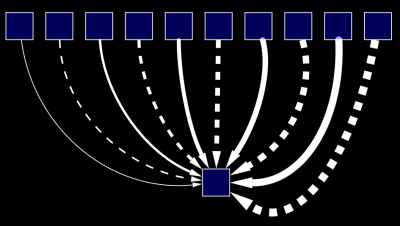
\includegraphics[width=.6\textwidth]{images/LineTypes.png} }
\end{itemize}

\item 用不同形状的节点表示不同的东西。\begin{itemize}
\item \centerline{
 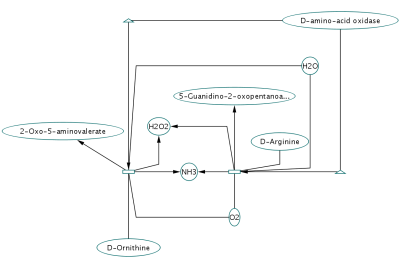
\includegraphics[width=.6\textwidth]{images/NodeShapeMapping.png}} 
\end{itemize}

\item 根据节点的度设置节点的大小。这样就能明显的看出hub节点\ldots\begin{itemize}
\item \centerline{
 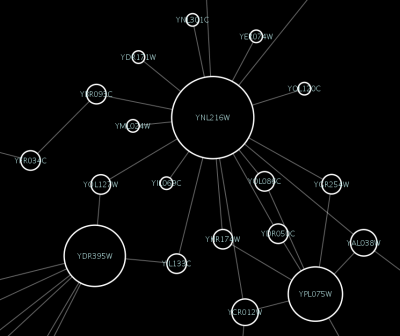
\includegraphics[width=.6\textwidth]{images/DegreeSize.png} }
\end{itemize}

\item \ldots或者设置节点标签的字体大小也能实现同样的目的。\begin{itemize}
\item \centerline{
 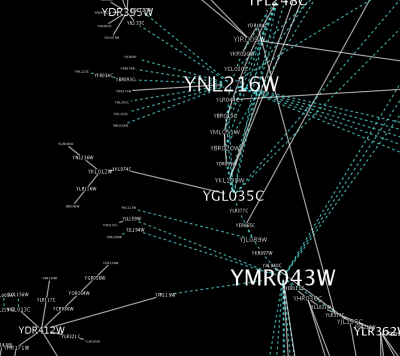
\includegraphics[width=.6\textwidth]{images/DegreeLabelSize.png} }
\end{itemize}

\item 根据标签的大小设置节点的宽度和高度。\begin{itemize}
\item \centerline{
 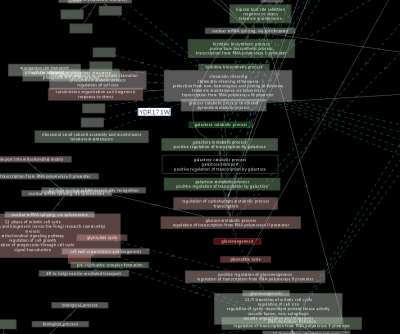
\includegraphics[width=.6\textwidth]{images/LabelWidthAndHeight.png}} 
\end{itemize}

\item 用渐变的颜色展示基因表达。\begin{itemize}
\item \centerline{
 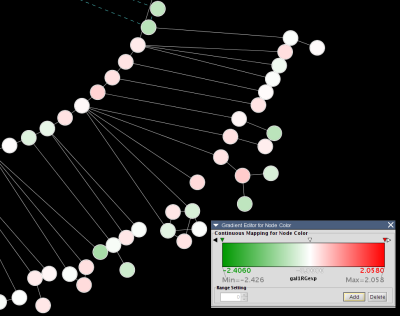
\includegraphics[width=.6\textwidth]{images/ColorGradient.png} }
\end{itemize}

\item 用边的权重控制边的透明度。\begin{itemize}
\item \centerline{
 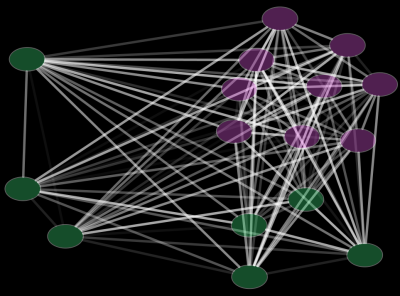
\includegraphics[width=.6\textwidth]{images/OpacityForEdges.png} }
\end{itemize}

\item 用边的分数控制边的多种视觉属性。\begin{itemize}
\item \centerline{
 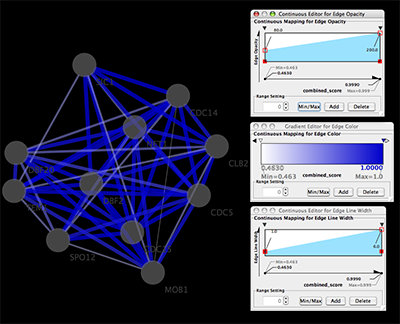
\includegraphics[width=.6\textwidth]{images/MultipleEdgeMapping.png} }
\end{itemize}

\item 通过调整节点的透明度观察高密度网络。\begin{itemize}
\item\centerline{
 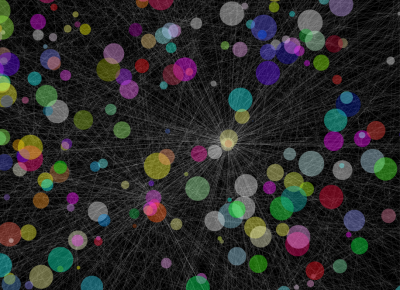
\includegraphics[width=.6\textwidth]{images/OpacityForNodesAndEdges.png} }
\end{itemize}

\item 显示网络中模块的位置。\begin{itemize}
\item \centerline{
 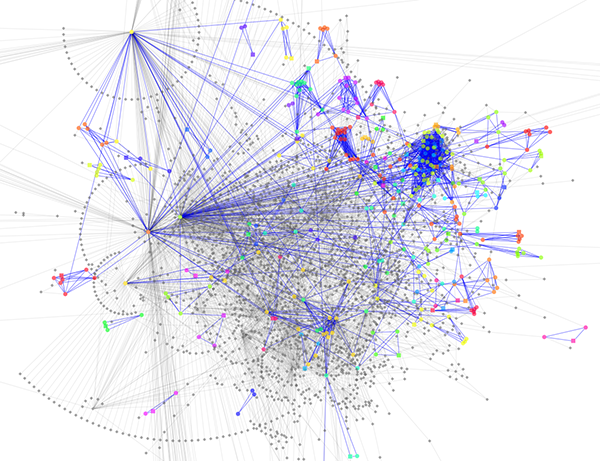
\includegraphics[width=.6\textwidth]{images/ModuleLocations.png} }
\end{itemize}

\item 利用透明度和颜色凸显整个网络的一个子网。\begin{itemize}
\item \centerline{
 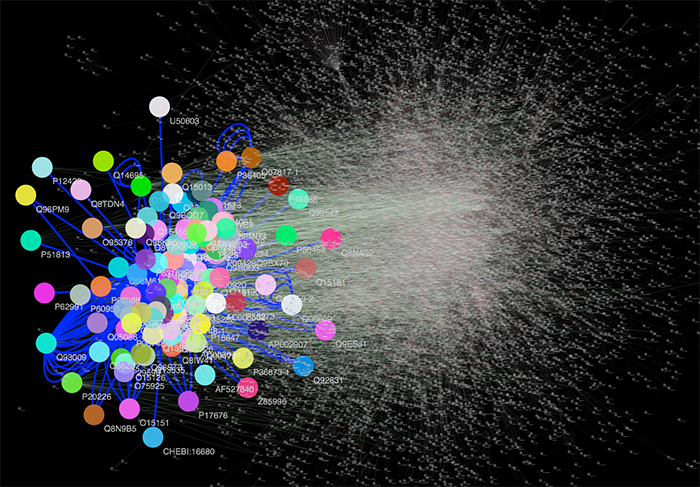
\includegraphics[width=.6\textwidth]{images/Overlay.png} }
\end{itemize}
\end{itemize}

Cytoscape 2.6.0及其以后的版本中有一些视觉风格的示例。通过这些示例可以大概了解到视觉风格对是如何影响网络的外观的。下面这些网络视图就是这些视觉风格的示例应用在\emph{galFiltered.sif}网络上的效果: 

 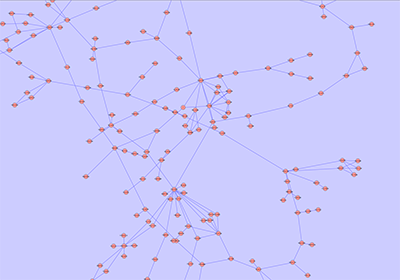
\includegraphics[width=.5\textwidth]{images/default_style.png}  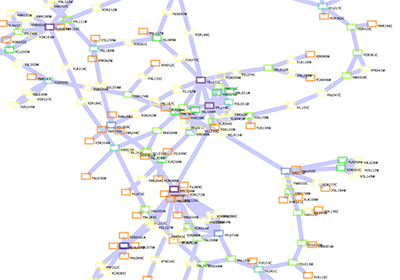
\includegraphics[width=.5\textwidth]{images/metro_style.png}  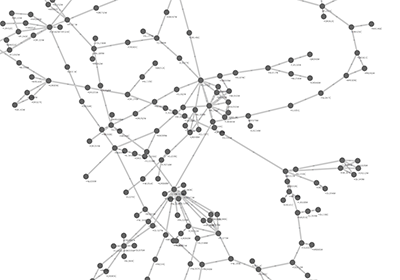
\includegraphics[width=.5\textwidth]{images/solid_style.png}  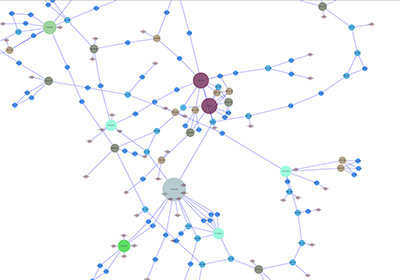
\includegraphics[width=.5\textwidth]{images/ripple_style.png}  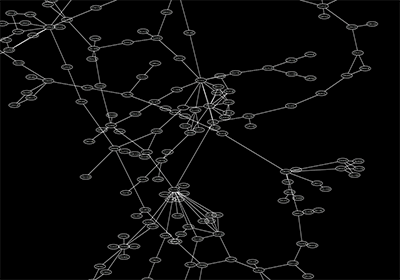
\includegraphics[width=.5\textwidth]{images/skeleton_style.png}  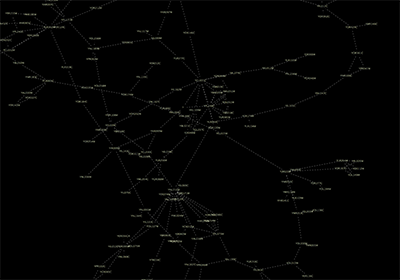
\includegraphics[width=.5\textwidth]{images/universe_style.png} 

通过View $\rightarrow$ Open VizMapper或是点击VizMapper图标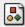
\includegraphics[width=1em]{images/VizMapIcon.png}就能启动VizMapper。此外,从2.5.0开始,在屏幕左侧的控制面板(以前称为CytoPanel 1)上有一个VizMapper的标签。
\section{VizMapper用户界面简介}
 As of Cytoscape 2.5, the VizMapper has undergone a complete interface redesign. There are three types of components in the new VizMapper: 
\begin{enumerate}
\item Main Panel 
\begin{itemize}
\item \centerline{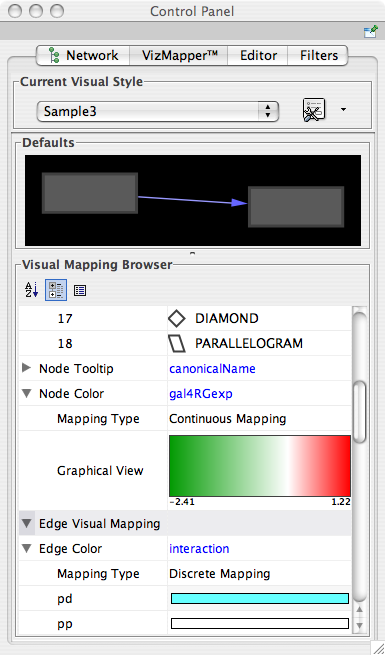
\includegraphics[width=.4\textwidth]{images/VizMapperMainPanel.png} }
\item This panel allows you to create/delete/view/switch between different visual styles using the Current Visual Style options. The Visual Mapping Browser at the bottom displays the mapping details for a given visual style and is used to edit these details as well. 
\end{itemize}

\item Default Appearance Editor \begin{itemize}
\item \centerline{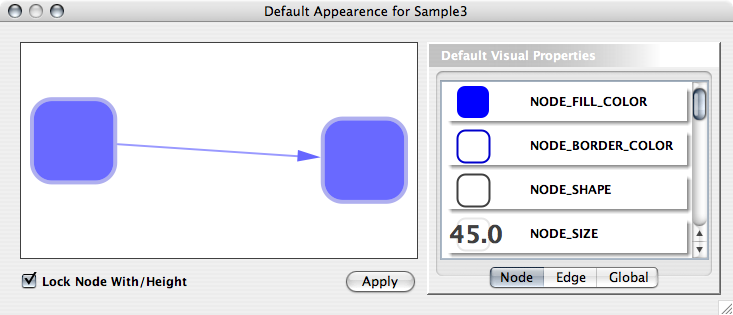
\includegraphics[width=.6\textwidth]{images/DefaultEditorPanel.png} }
\item Clicking on the section labelled ``Defaults'' on the Main Panel will bring up this editor, which allows users to visually edit the default appearance of nodes and edges for the selected visual style. 
\end{itemize}

\item Continuous Editors \begin{itemize}
\item These are editors for continuous mapping, which is a mapping from numerical value to visual attributes. They are accessed through the Visual Mapping Browser on the Main Panel. Using these windows, users can edit continuous mapping more intuitively. 
\item Color Gradient Editor 
\item Continuous-to-Discrete Editor 
\item Continuous-to-Continuous Editor 
\end{itemize}

\end{enumerate}
 These editors will be discussed in further detail below. 
\section{Introduction to Visual Styles}
The Cytoscape distribution includes several predefined visual styles to get you started. To demonstrate these styles, try out the following example: 

\textbf{Step 1. Load some sample data}

\begin{itemize}
\item 

 Load a sample session file: From the main menu, select \emph{\textbf{File \^a†’ Open}
}
, and select the file \emph{sampleData/galFiltered.cys}
. 

\item 

 The session file includes a network, some annotations, and sample visual styles. By default, \textbf{galFiltered Style}
 is selected. Gene expression values for each node will be colored along a color gradient between red and green (where red represents a low expression ratio and green represents a high expression ratio, using thresholds set for the gal4RGexp experiment bundled with Cytoscape in the \emph{sampleData/galExpData.pvals}
 file). Also, node size is mapped onto the degree (number of edges connected to the node) and you can see the hubs of the network as larger nodes. See the sample screenshot below: 


 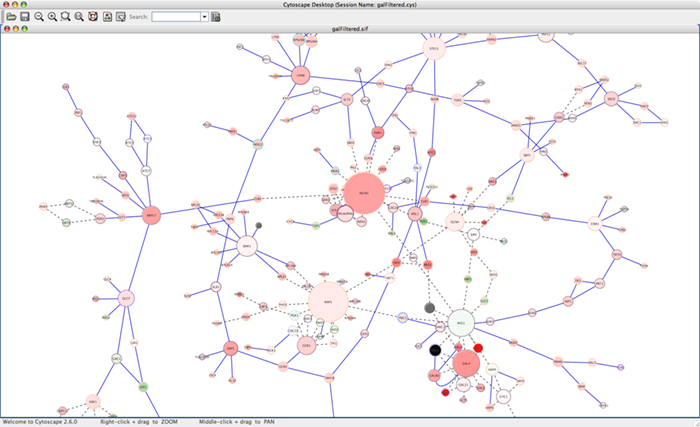
\includegraphics[width=.6\textwidth]{images/galFilteredSessionDefault.png} 


\end{itemize}


 \textbf{Step 2. Switch between different Visual Styles}



 You can change visual styles by making a selection from the Current Visual Style dropdown list (found at the top of the VizMapper Main Panel). 


 For example, if you select \textbf{Sample1}
, a new visual style will be applied to your network, and you will see a white background and round blue nodes. Additionally, if you zoom in closer, you can see that protein-DNA interactions (specified with the label ``pd'') are drawn with dashed red edges, whereas protein-protein interactions (specified with the label ``pp'') are drawn with a solid light blue edge (see sample screenshot below). 
\begin{itemize}
\item 

 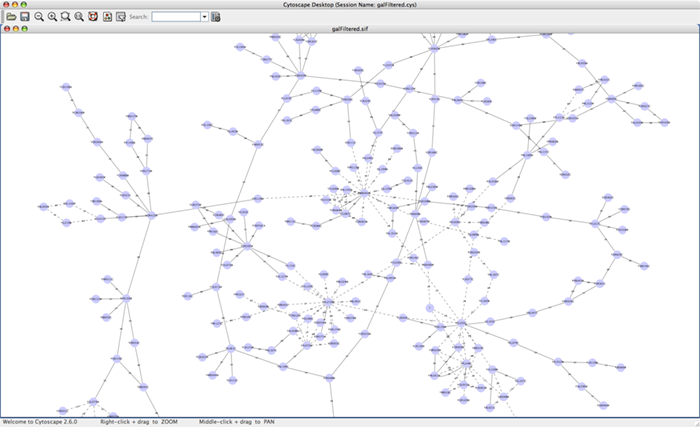
\includegraphics[width=.6\textwidth]{images/VizMapperSample1Style26.png} 


\end{itemize}


 Finally, if you select \textbf{Solid}
, you can see the graphics below: 
\begin{itemize}
\item 

 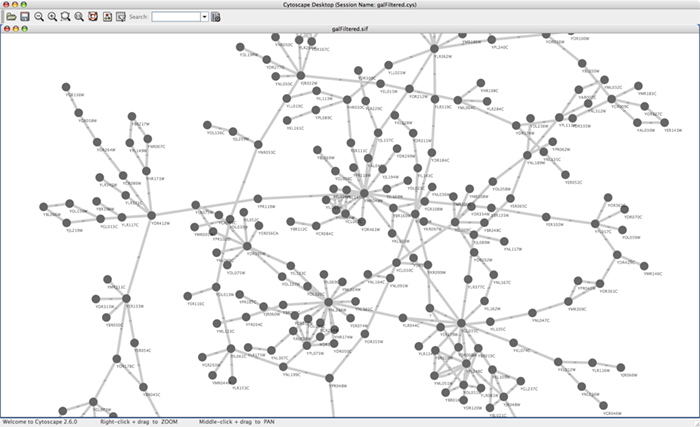
\includegraphics[width=.6\textwidth]{images/VizMapperSolidStyle.png} 


\end{itemize}


 This Visual Style does not have mappings except node/edge labels, but you can modify the network graphics by editing \emph{Default View}
. 


 Additional sample styles are available as \emph{sampleStyles.props}
 file in the \emph{SampleData}
 directory. You can import the sample file from \emph{\textbf{File \^a†’ Import \^a†’ Vizmap Property File}
}
. 


 
\section*{Visual Attributes, Graph Attributes and Visual Mappers}


 The Cytoscape VizMapper uses three core concepts: 
\begin{itemize}
\item 

 A \emph{visual attribute}
 is any visual setting that can be applied to your network. For example, you can change all nodes from circles to squares by changing the node shape visual attribute. 

\item 

 A \emph{network attribute}
 is any data attribute associated with a node or an edge. For example, each edge in a network may be associated with a label, such as \^a€œpd\^a€ (protein-DNA interactions), or \^a€œpp\^a€ (protein-protein interactions). 

\item 

A \emph{visual mapper}
 maps network attributes to visual attributes. For example, a visual mapper can map all protein-DNA interactions to the color blue, and all protein-protein interactions to the color red. 
\end{itemize}
Cytoscape allows a wide variety of visual attributes to be controlled. These are summarized in the tables below. 

\textbf{Table 18}\\
\begin{center}
\begin{tabular}{|c|}
\hline
 \textbf{Visual Attributes Associated with Nodes} \\
\hline
 Node Color \\
\hline
 Node Opacity \\
\hline
 Node Border Color \\
\hline
 Node Border Opacity \\
\hline
 Node Border Line Style. \\
Solid and dashed lines are supported.  \\
\hline
 Node Border Line Width \\
\hline
 Node Shape. \\The following options are available: \\
\hline
 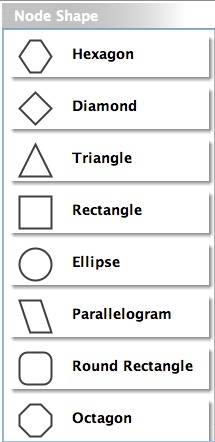
\includegraphics[width=.2\textwidth]{images/NewVizMapperNodeShape.png} \\
\hline
 Node Size: the width and height of each node.  \\
\hline
 Node Label: the text label for each node.  \\
\hline
 Node Label Color \\
\hline
 Node Label Opacity \\
\hline
 Node Label Position:\\ the position of the label relative to the node.  \\
\hline
 Node Font: node label font and size. \\
 \hline 
\end{tabular}
%\textbf{Table 19}\\
\begin{tabular}{|c|}
\hline 
\textbf{Visual Attributes Associated with Edges}\\
\hline 
Edge Color \\
\hline 
Edge Opacity \\
\hline 
Edge Line Style.\\ Solid or dashed lines are supported.\\
\hline 
Edge Line Width\\ 
\hline 
Edge Source and Target Arrow Shape:\\
The following options are available: \\
\hline 
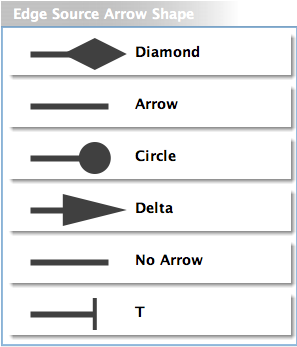
\includegraphics[width=.3\textwidth]{images/NewVizMapperArrowType.png} \\
\hline 
Edge Source and Target Arrow Color \\
\hline 
Edge Source and Target Arrow Opacity \\
\hline 
Edge Label: the text label for each edge. \\
\hline 
Edge Label Color \\
\hline 
Edge Label Opacity \\
\hline 
Edge Font: edge label font and size.\\
\hline 
\end{tabular}
\end{center}

\textbf{Table\^A 20.\^A }
\begin{tabular}{|c|c|c|c|}
\hline 
 \textbf{Global Visual Properties} & Background Color & Selected Node Color & Selected Edge Color \\
 \hline 
\end{tabular}


 For each visual attribute, you can specify a default value or define a dynamic visual mapping. Cytoscape currently supports three different types of visual mappers: 
\begin{enumerate}
\item \textbf{Passthrough Mapper}
\begin{itemize}
\item The values of network attributes are passed directly through to visual attributes. A passthrough mapper is only used to specify node/edge labels. For example, a passthrough mapper can label all nodes with their common gene names. 
\end{itemize}

\item \textbf{Discrete Mapper}
\begin{itemize}
\item Discrete network attributes are mapped to discrete visual attributes. For example, a discrete mapper can map all protein-protein interactions to the color blue. 
\end{itemize}

\item \textbf{Continuous Mapper}
\begin{itemize}
\item Continuous graph attributes are mapped to visual attributes. Depending on the visual attribute, there are three kinds of continuous mappers: \begin{enumerate}
\item \textbf{Continuous-to-Continuous Mapper}: for example, you can map a continuous numerical value to a node size. 
\item \textbf{Color Gradient Mapper}: This is a special case of continuous-to-continuous mapping. Continuous numerical values are mapped to a color gradient. 
\item \textbf{Continuous-to-Discrete Mapper}: for example, all values below 0 are mapped to square nodes, and all values above 0 are mapped to circular nodes. 
\end{enumerate}

\item However, note that there is no way to smoothly morph between circular nodes and square nodes. 
\end{itemize}
\end{enumerate}


 The table below shows visual mapper support for each visual property. 

 \textbf{Legend}

 \textbf{Table 21}
\begin{tabular}{|c|c|c|c|}
\hline 
\textbf{Symbol} \textbf{Description} &
Mapping is not supported for the specified visual property.  &
X Mapping is fully supported for the specified visual property.  &
o Mapping is partially supported for the specified visual property. Support for \^a€œcontinuous to continuous\^a€ mapping is not supported.  \\
\hline 
\end{tabular}

\textbf{Node Visual Mappings}

 \textbf{Table 22}
\begin{tabular}{|c|c|c|c|c|c|c|c|c|c|c|c|c|c|c|}
\hline 
 \textbf{Node Visual Properties}

 \textbf{Passthrough Mapper}

 \textbf{Discrete Mapper}

 \textbf{Continuous Mapper}

\^A  &

 Color


  Node Color 


  - 


  X 


  X 
 &

  Node Opacity 


  - 


  X 


  X 
\^A  &

  Node Border Color 


  - 


  X 


  X 
\^A  &

  Node Border Opacity 


  - 


  X 


  X 
\^A  &

  Node Label Color 


  - 


  X 


  X 
\^A  &

  Node Label Opacity 


  - 


  X 


  X 
\^A  &

 Numeric 


  Node Size 


  - 


  X 


  X 
 &

  Node Font Size 


  - 


  X 


  X 
\^A  &

  Node Line Width 


  - 


  X 


  X 
\^A  &

 Other


  Node Border Type 


  - 


  X 


  o 
 &

  Node Shape 


  - 


  X 


  o 
\^A  &

  Node Label 


  X 


  X 


  o 
\^A  &

  Node Tooltip 


  X 


  X 


  o 
\^A  &

  Node Font Family 


  - 


  X 


  o 
\^A  \\
 \hline 

\end{tabular}



 \textbf{Edge Visual Mappings}



 \textbf{Table\^A 23.\^A }



\begin{tabular}{|c|c|c|c|c|c|c|c|c|c|c|c|c|c|c|c|c|}
\hline 
 & & & & & & & & & & & & & & & & \\
 \hline 


 \textbf{Edge Properties}



 \textbf{Passthrough Mapper}



 \textbf{Discrete Mapper}



 \textbf{Continuous Mapper}

\^A  &

 Color


 Edge Color 


 - 


 X 


 X 
 &

 Edge Opacity 


 - 


 X 


 X 
\^A  &

 Edge Target Arrow Color 


 - 


 X 


 X 
\^A  &

 Edge Source Arrow Color 


 - 


 X 


 X 
\^A  &

 Edge Target Arrow Opacity 


 - 


 X 


 X 
\^A  &

 Edge Source Arrow Opacity 


 - 


 X 


 X 
\^A  &

 Edge Label Color 


 - 


 X 


 X 
\^A  &

 Edge Label Opacity 


 - 


 X 


 X 
\^A  &

 Numeric


  Edge Line Width 


 - 


 X 


 X 
 &

 Edge Font Size 


 - 


 X 


 X 
\^A  &

 Other 


  Edge Line Type 


  - 


 X 


 o 
 &

  Edge Source Arrow Shape 


  - 


  X 


  o 
\^A  &

  Edge Target Arrow Shape 


  - 


 X 


 o 
\^A  &

  Edge Label 


  X 


  X 


 o 
\^A  &

  Edge Tooltip 


  X 


  X 


 o 
\^A  &

  Edge Font Family 


  - 


 X 


 o 
\^A  \\
 \hline 

\end{tabular}



 
\section*{Visual Styles Tutorials}


 The following tutorials demonstrate some of the basic VizMapper features. Each tutorial is independent of the others. 


 \textbf{Tutorial 1: Create a Basic Visual Style and Set Default Values}


 The goal of this tutorial is to learn how to create a new Visual Style and set some default values. 


 \textbf{Step 1. Load a sample network.}
 From the main menu, select File \^a†’ Import \^a†’ Network (Multiple file types), and select sampleData/galFiltered.sif. 


 \textbf{Step 2. Open the VizMapper.}
 Select the View \^a†’ Open VizMapper menu option, or select the VizMapper icon in the main button bar, or click on the VizMapper tab in the Control Panel at the left of the screen. You will now see a VizMapper Main Panel, as shown below. 
\begin{itemize}
\item 

 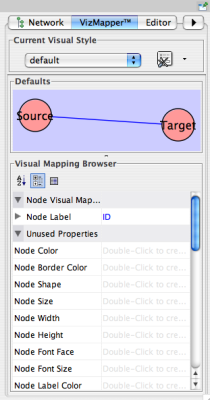
\includegraphics[width=.4\textwidth]{images/NewVizMapper.png} 


\end{itemize}


 \textbf{Step 3. Create a new visual style.}
 Click the Options 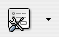
\includegraphics[width=1em]{images/VizMapOptionIcon.png}  button, and select \emph{Create new visual style...}
 Then enter a name for your new visual style when prompted. You will see an empty visual style in the VizMapper Main Panel, as shown below. 
\begin{itemize}
\item 

 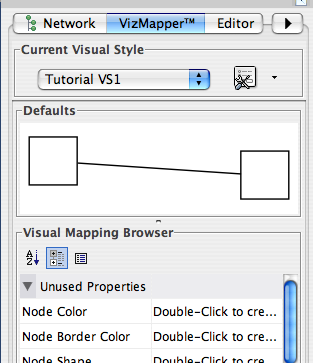
\includegraphics[width=.6\textwidth]{images/EmptyVisualStyle.png} 


\end{itemize}


 Since no mapping is set up yet, all visual attributes are listed in the Unused Properties category. From this panel, you can create node/edge mappings for all visual properties. 


 \textbf{Step 4. Edit default values.}
 Open the Default Appearance Editor by clicking on the Defaults graphics window (shown below) in the VizMapper Main Panel. 
\begin{itemize}
\item 

 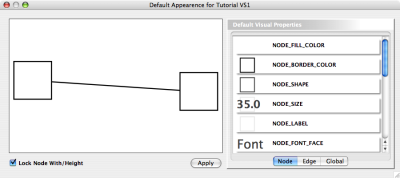
\includegraphics[width=.6\textwidth]{images/InitialDefaultEditor.png} 


\end{itemize}


 \textbf{Step 5. Change the default node shape.}
 To set the default node shape to triangles, click ``Node Shape'' in the Default Visual Properties list. A list of available node shapes will be shown. Click on the Triangle icon and then click the Apply button. The Default Appearance Editor will be automatically updated. You can edit other default values by clicking on visual attribute names on the list. In the example shown below, the node shape is set to Triangle, while the node color is set to blue. 
\begin{itemize}
\item 

 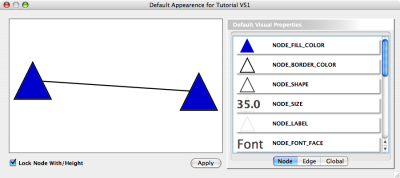
\includegraphics[width=.6\textwidth]{images/TriangleDefaultEditor.png} 


\end{itemize}


 \textbf{Step 6. Apply your settings.}
 When you finish editing, click the Apply button at the bottom of the editor. Your new Visual Style will be applied to the current network, as shown below. 
\begin{itemize}
\item 

 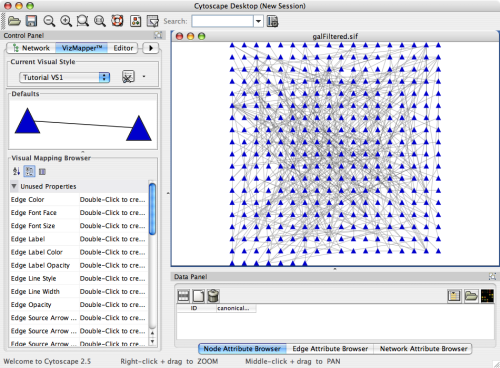
\includegraphics[width=.6\textwidth]{images/Tut1GalFiltered.png} 


\end{itemize}


 
\textbf{Tutorial 2: Creating a New Visual Style with a Discrete Mapper}


 The following tutorial demonstrates how to create a new visual style using a discrete mapper. The goal is to draw protein-DNA interactions as dashed blue lines, and protein-protein interactions as solid red lines. 


 \textbf{Step 1. Load a sample network.}
 From the main menu, select File \^a†’ Import \^a†’ Network (Multiple file types), and select sampleData/galFiltered.sif. 


 \textbf{Step 2. Open the VizMapper.}
 Select the View \^a†’ Open VizMapper menu option, or select the VizMapper icon in the main button bar, or click on the VizMapper tab in the Control Panel at the left of the screen. 


 \textbf{Step 3. Create a new visual style.}
 Click the Options 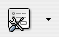
\includegraphics[width=.6\textwidth]{images/VizMapOptionIcon.png}  button, and select \emph{Create new visual style...}
 Name your new style \^a€œTutorial VS2\^a€. 


 \textbf{Step 4. Choose a visual attribute.}
 Double click the Edge Color entry listed in Unused Properties. Edge Color will now appear at the top of the list, under the Edge Visual Mapping category (as shown below). 
\begin{itemize}
\item 

 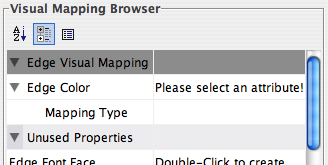
\includegraphics[width=.6\textwidth]{images/EdgeMapping1.png} 


\end{itemize}


 \textbf{Step 5. Choose a network attribute.}
 Click on the cell to the right of the Edge Color entry and select ``interaction'' from the dropdown list that appears. 


 \textbf{Step 6. Choose a mapping type.}
 Set the Discrete Mapper option as the Mapping Type. All available attribute values for ``interaction'' will be displayed, as shown below. 
\begin{itemize}
\item 

 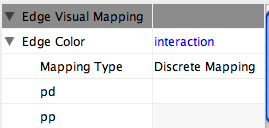
\includegraphics[width=.6\textwidth]{images/EdgeMapping2.png} 


\end{itemize}


 \textbf{Step 7. Set the mapping relationship.}
 Click the empty cell next to ``pd'' (protein-DNA interactions). On the right side of the cell, \textbf{...}
 and \textbf{X}
 buttons will appear. Click on the \textbf{...}
 button. A popup window will appear; select blue, and the change will immediately appear on the network window. 
\begin{itemize}
\item 

 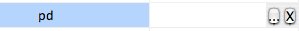
\includegraphics[width=.6\textwidth]{images/CellEditor1.png} 


\end{itemize}


 Repeat step 7 for ``pp'' (protein-protein interactions), but select red as the edge color. Then repeat steps 4 through 7 for the Edge Line Style attribute. You can select the correct line style (dashed or solid) from the dropdown list. 
\begin{itemize}
\item 

 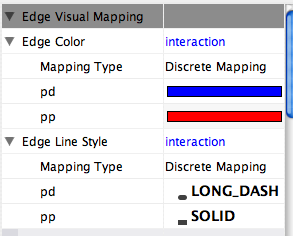
\includegraphics[width=.6\textwidth]{images/EdgeMapping3.png} 


\end{itemize}


 Now your network should show ``pd'' interactions as dashed blue lines and ``pp'' interactions as solid red lines. A sample screenshot is provided below. 


 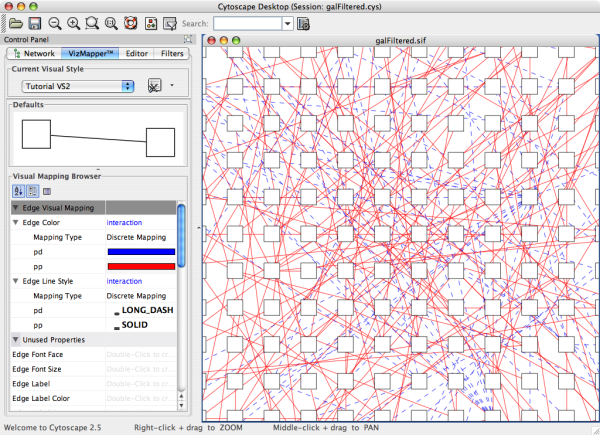
\includegraphics[width=.6\textwidth]{images/NewVizMapperInteractionsRedBlue.png} 


 
\textbf{Tutorial 3: Visualizing Expression Data on a Network}


 The following tutorial demonstrates how to create a new visual style using a continuous mapper. The goal is to superimpose gene expression data onto a network and display gene expression values along a color gradient. 


 \textbf{Step 1. Load a sample network.}
 From the main menu, select File \^a†’ Import \^a†’ Network (Multiple file types), and select sampleData/galFiltered.sif. 


 \textbf{ Step 2. Load sample expression data.}
 From the main menu, select File \^a†’ Import \^a†’ Attribute/Expression Matrix, and select sampleData/galExpData/pvals. 


 \textbf{Step 3. Open the VizMapper.}
 Select the View \^a†’ Open VizMapper menu option, or select the VizMapper icon in the main button bar, or click on the VizMapper tab in the Control Panel at the left of the screen. 


 \textbf{Step 4. Create a new visual style.}
 Click the Options 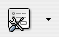
\includegraphics[width=.6\textwidth]{images/VizMapOptionIcon.png}  button, and select \emph{Create new visual style...}
 Name your new style \^a€œTutorial VS3\^a€. 


 \textbf{Step 5. Choose a visual attribute.}
 Double click the Node Color entry listed in Unused Properties. Node Color will now appear at the top of the list, under the Node Visual Mapping category. 


 \textbf{Step 6. Choose a network attribute.}
 Click on the cell to the right of the Node Color entry and select ``gal1RGexp'' from the dropdown list that appears. 


 \textbf{Step 7. Choose a mapping type.}
 Set the Continuous Mapping option as the Mapping Type. This automatically creates a default mapping 
\begin{itemize}
\item 

 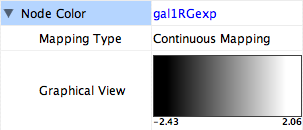
\includegraphics[width=.6\textwidth]{images/DefaultColorGradient.png} 


\end{itemize}


 \textbf{Step 8. Define the points where colors will change.}
 Double-click on the black-and-white gradient rectangle next to Graphical View to open the Color Gradient Mapper. Click and drag one point to -1, or type the value in the Range Setting box. Set the second point to 2. 
\begin{itemize}
\item 

 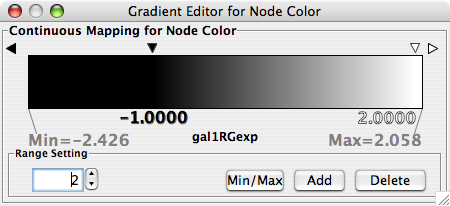
\includegraphics[width=.6\textwidth]{images/DefaultColorGradientEditor.png} 


\end{itemize}


 \textbf{Step 9. Define the colors between points.}
 Double-click on the leftmost triangle (facing left) and a color palette will appear. Choose a shade of yellow and click OK. Double-click on the triangle at -1 and set the color white. For triangle at 2, set its color to red. Set the rightmost triangle to black. 
\begin{itemize}
\item 

 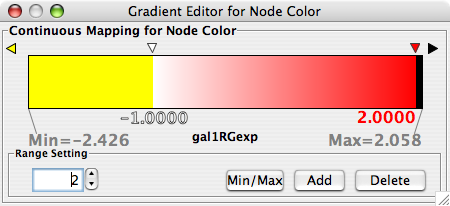
\includegraphics[width=.6\textwidth]{images/RedYellowColorGradient2.png} 


\end{itemize}


 The color gradients will immediately appear in the network window. All nodes with a gal1RGexp value less than \^a€“1 will be set to yellow, and all nodes with a gal1RGExp value greater than 2 will be black. Additionally, all values between \^a€“1 and 2 will be painted with a white/red color gradient. A sample screenshot is below. 


 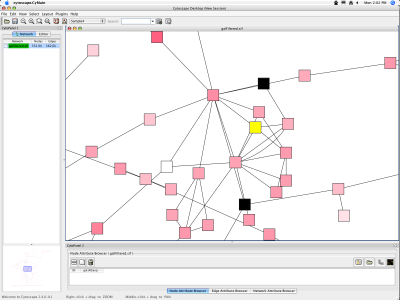
\includegraphics[width=.6\textwidth]{images/VizMapperExpRedBlack.png} 


 
\textbf{Tutorial 4: How to Use Utilities for Discrete Mappers}


 The following tutorial demonstrates new features in Cytoscape 2.5. The new VizMapper user interface has some utilities to help users editing discrete mappings. The goal of this section is learning how to set and adjust values for discrete mappings automatically. 
\begin{enumerate}
\item 

 Load a sample network: From the main menu, select File \^a†’ Import \^a†’ Network, and select sampleData/galFiltered.sif. 

\item 

 Apply layout to the network: From the main menu, select Layout \^a†’ Cytoscape Layouts \^a†’ Degree Sorted Circle Layout. This layout algorithm sort nodes in a circle by degree of the nodes. Degrees will be stored as node attribute names \emph{Degree}
 after you applied this algorithm. 

\item 

 Click the VizMap 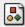
\includegraphics[width=.6\textwidth]{images/VizMapIcon.png}  button on the tool bar. 

\item 

 Click \emph{Defaults}
 panel on the VizMapper main panel. Default Apearence Editor pops up (see below.) 

\item 

 Edit the following visual properties and press \emph{\textbf{Apply}
}
. Since you changed opacity of the node, you can see the nodes bihind the front node (see below.) 
\begin{itemize}
\item Node Oppacity - 100 
\item Edge Color - White 
\item Background Color - Black 

\end{itemize}


 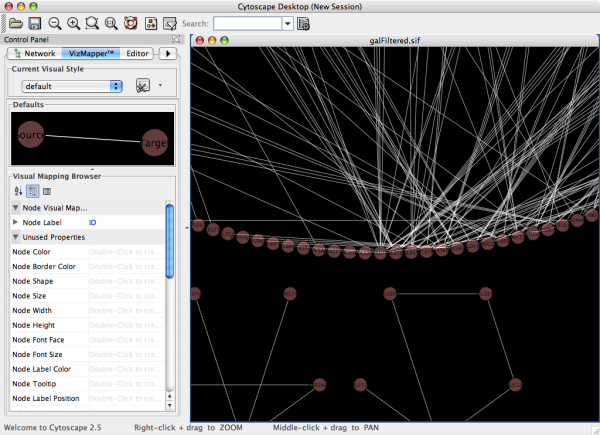
\includegraphics[width=.6\textwidth]{images/Opacity1.png} 

\item 

 Cretate a \textbf{Discrete Node Color Mapping}
. Select \emph{Degree}
 as controlling attribute. 

\item 

 Select \textbf{Node Color}
, then right click to show popup menu. Select Generate discrete values \^a†’ Rainbow 1. It generates different colors for different attribute values as shown below. 


 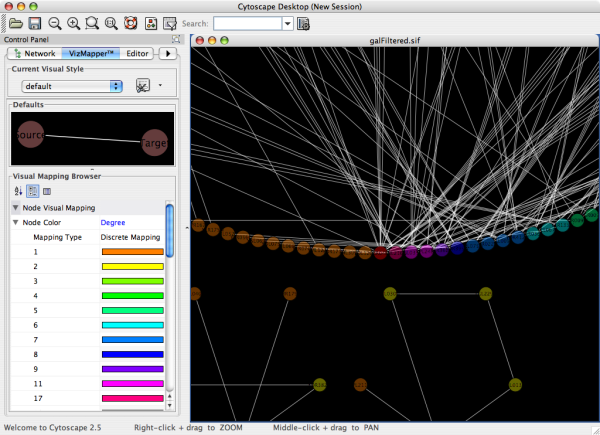
\includegraphics[width=.6\textwidth]{images/Rainbow1.png} 

\item 

 Cretate a \textbf{Discrete Node Size Mapping}
. Select \emph{Degree}
 as controlling attribute. 

\item 

 Select \textbf{Node Size}
 and right click to show popup menu. Select Generate Discrete Values \^a†’ Series (Numbers Only). Type \emph{30}
 for the first value and click OK. Enter \emph{15}
 for increment. 

\item Apply Force-Directed layout. Final view of the window looks like the following. 

 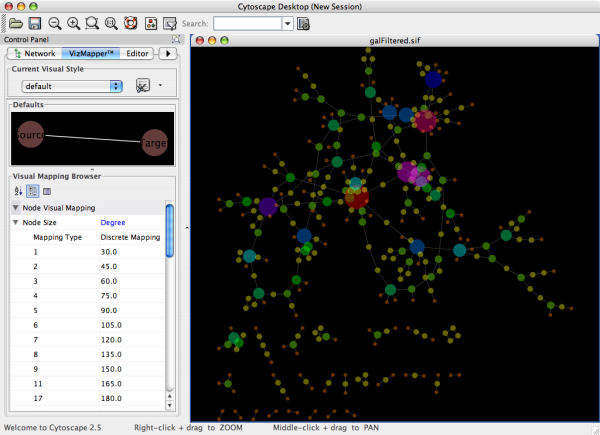
\includegraphics[width=.6\textwidth]{images/tutorial4_last.png} 


\end{enumerate}


 

\section*{Advanced Topics}


 \textbf{Editing Discrete Mappings}


 From version 2.5, several utility functions are available for Discrete Mappings. You can use those functions by right clicking anywhere on the \emph{Visual Mapping Browser}
 (shown below.) 


 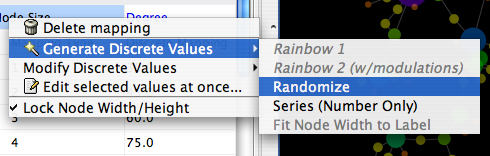
\includegraphics[width=.6\textwidth]{images/VizMapperPopupMenu.png} 


 \textbf{Automatic Value Generators}
\begin{itemize}
\item 

 \emph{\textbf{Generate Discrete Values}
}
 - Functions in this menu category are value generator for discrete mappings. Users can set values for discrete mappings automatically by these functions. 
\begin{itemize}
\item 

 \textbf{Rainbow 1}
 and \textbf{Rainbow 2}
 - These functions try to assign as different colors as possible to each values. see the example below: 
\begin{itemize}
\item 

 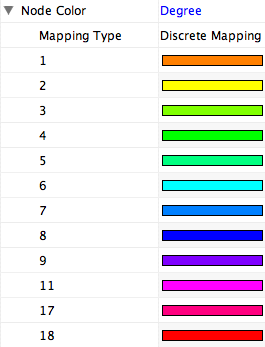
\includegraphics[width=.6\textwidth]{images/RainbowExample1.png} 


\end{itemize}

\item 

 \textbf{Randomize}
 - Randomize colors and numbers. If you use this function for numerical values (node size, opacity, etc.) you need to specify a range. For example, if you want to set values from 1 to 100, you need to type \emph{1-100}
 in the dialog. 

\item 

 \textbf{Series}
 - Set series of numbers to the specified mapping. 
\begin{itemize}
\item 

 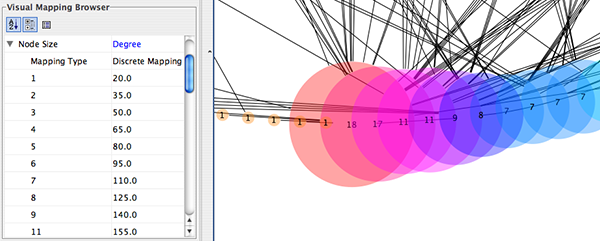
\includegraphics[width=.6\textwidth]{images/SeriesExample1.png} 


\end{itemize}

\item 

 \textbf{Fit node size to label}
 - This function is only for node width and height. When node size is \emph{unlocked}
 AND \emph{Node Width/Height}
 discrete mappings are available, you can fit the size of each node to label automatically by selecting this function. See the example below: 
\begin{itemize}
\item 

 \includegraphics[width=.6\textwidth]{images/NodeLabelFit.png} 


\end{itemize}


\end{itemize}

\item 

 \emph{\textbf{Modify Discrete Values}
}
 - Currently, this is only for colors. You can change overall brightness for discrete color mappings. 


\end{itemize}


 
\textbf{Edit Selected Values at Once}


 You can set multiple values at once. First, you need to select rows you want to change values then select \emph{Edit selected values at once...}
. A dialog pops up and you can enter the new value for the selected rows. 


 
\textbf{Lock Node Width/Height}


 If this menu item is checked, \emph{Node Width}
 and \emph{Node Height}
 mappings are ignored and \emph{Node Size}
 overrides them. If you want to use \emph{Fit node size to label}
 function, you need to unlock this. 


 

\textbf{Working with Continuous Mapping Editors}


 There are three kinds of Continuous Mapping Editors. Each of them are associated with a specific visual attributes: 


 \textbf{Table\^A 24.\^A }



\begin{tabular}{|c|c|c|c|}
\hline 
 & & & \\
 \hline 


 \emph{\textbf{Editor Type}
}



 \emph{\textbf{Supported Data Type}
}



 \emph{\textbf{Visual Attributes}
}

 &

 \textbf{Color Gradient Editor}



  Color 


  node/edge/border/label colors 
 &

 \textbf{Continuous-Continuous Editor}



  Numbers 


  size/width/opacity 
 &

 \textbf{Continuous-Discrete Editor}



  All others 


  font/shape/text 
 \\
 \hline 

\end{tabular}


 \textbf{Range Setting Panel}


 \includegraphics[width=.6\textwidth]{images/RangeSetting26.png} 


 Each editor has a common section named \emph{\textbf{Range Setting}
}
. 
\begin{enumerate}
\item 

 \textbf{Handle Value Box}
 - This box displays current value for selected slider handle. Also you can directly type value in this box to move the slider to exact location. 

\item 

 \textbf{Min/Max Button}
 - Set the overall range of this editor. First time you open the editor, the \emph{Min}
 and \emph{Max}
 values are set by the range of attribute you selected, i.e., minimum and maximum value of the attribute will be set to the range of this editor. You can change this range anytime you want by pressing this button. 

\item 

 \textbf{Add Handle Button}
 - Add a new handle to the editor. 

\item 

 \textbf{Delete Handle Button}
 - Delete selected handle from the slider widget. 


\end{enumerate}


 
\textbf{Gradient Editor}


 \includegraphics[width=.6\textwidth]{images/GradientEditorSample26.png} 


 Gradient Editor is a editor to create continuous mapping for colors. To change the color of each region, just double click the handles (small triangles on the top). Color gradient will be created only when editor has two or more handles (see the example below). 


 \textbf{Table\^A 25.\^A }



\begin{tabular}{|c|c|}
\hline 
 & \\
 \hline 


  1 Slider (No Graient) 


  2 Sliders 
 &

 \includegraphics[width=.6\textwidth]{images/OneSlider.png} 


 \includegraphics[width=.6\textwidth]{images/TwoSliders.png} 
 \\
 \hline 

\end{tabular}


 
\textbf{Continuous-Continuous Editor}


 \includegraphics[width=.6\textwidth]{images/C2CEditor26.png} 


 Continuous-Continuous Editor is for creating mapping between numerical attributes and numerical visual properties (size/opacity). To change the value assigned on Y-axis (visual property shown in the example above is node size), drag the red squares or double click on the squares to directly type exact value. 


 
\textbf{Continuous-Discrete Editor}


 \includegraphics[width=.6\textwidth]{images/C2DEditor26.png} 


 Continuous-Discrete Editor is used to create mapping from numerical attribute values to discrete visual properties, such as font, shape, or line style. To edit a value for specific region, double click on the icon on the track. 


 

\section*{Managing Visual Styles}


 All Cytoscape Visual Style settings are initially loaded from a a default file called vizmap.props that cannot be altered by users. When users make changes to the visual properties, a vizmap.props file is saved in the session file. This means that assuming you save your session, you will not lose your visual properties. No other vizmap.props files are saved during normal operation. 


 \textbf{Saving Visual Styles}


 Visual styles are automatically saved with the session they were created in. Before Cytoscape exits, you will be prompted to make sure you save the session before quitting. It is also possible to save your visual styles in a file separate from the session file. To do this, navigate to the File \^a†’ Export \^a†’ Vizmap Property File menu option and save the properties as a file. This feature can be used to share visual styles with other users. 


 
\textbf{Importing Visual Styles}


 To import existing visual styles, navigate to the File \^a†’ Import \^a†’ Vizmap Property File menu option and select a vizmap.props file. Imported properties will supplement existing properties or override existing properties if the properties have the same name. You can also specify a visual properties file using the -V command line option (cytoscape.sh -V myVizmap.props). Visual properties loaded from the command line will override any default properties. 


 
\textbf{Default Visual Styles}


 It is possible to change the default visual properties for all sessions of Cytoscape. To do this, navigate to the Edit \^a†’ Preferences \^a†’ Properties... menu option, check the ``Make Current Visual Styles Default'' box in the Default Visual Styles section, and click the OK button. This will save the current visual styles as a vizmap.props file to your .cytoscape directory (found in your home directory). These visual styles will then be loaded each time Cytoscape is started. 


 

\section*{Bypassing Visual Styles}


 Cytoscape has a feature that allows users to override visualizations created by the VizMapper for individual nodes and edges. This feature is available by right-clicking on a node or edge and then clicking on the Visual Mapping Bypass menu. 

\includegraphics[width=.6\textwidth]{images/VizmapBypass26.png} 


 Each visual property of the node or edge is displayed. When a property is overridden, a checkmark appears next to the property and a [Reset $<$Property Name$>$] menu option appears directly below it. By clicking this Reset option, the bypass will be removed and the attribute will be displayed as defined by the VizMapper. At the bottom of the menu a Reset All option appears. When clicked, this will remove all bypasses for the specified node or edge. In the example above, you can see the the selected node size, color, and shape have been overridden. This is apparent in the appearance of the node itself and by the check marks in the popup menu. 


 It is important to realize that the the Visual Mapping Bypass only works for individual nodes and edges and not for all nodes or edges of a specific type. Using the bypass function is not particularly resource intensive, meaning you can use it as much as you like. However, if you ever find yourself repeating the same bypasses, then you should consider using the VizMapper instead. 


 Bypass is accomplished using special attributes with names like node.fillColor and node.shape. These are normal Cytoscape attributes and can be seen and edited in the Attribute Browser. The value of the attribute is a string representation of a property. For example, color is represented by 3 integers representing the RGB (red, green, blue) value of the color. Different types of properties have different string representations. When in doubt, just use the right click menu to create valid attribute values. 


 Because bypass values are specified using normal attributes, these attributes will persist between sessions only as long as you save your session! If you don't save your session, you will lose whatever bypass values you set. 
